\chapter{The Mu2e Tracker}\label{chaptertrk}
\section{Tracker panels}
\section{Tracker Front-End Electronics}
Before being accessible to the Mu2e Data Acquisition (DAQ) system, the analog signals from the Tracker straw tube channels need amplification, digitization and packaging. The Tracker front-end electronics (FEEs) are designed to achieve these goals. The FEEs consist of multiple Printed Circuit Boards (PCBs) as shown in Figure \ref{fig:trackerfee} \cite{vadimmu2e}.
All PCBs are situated in the outer section of the panel. Pulse timing is measured at the end of each straw, in order to be able to measure electron position on the wire. A measure of $dE/dx$ is provided, so pattern recognition can be possible \cite{bartoszek2015mu2e}. For this purpose each straw has:
\begin{itemize}
    \item 2 preamp channels, 1 for each end;
    \item 2 TDC channels, 1 for each end;
    \item 1 ADC channel, measuring sum of both ends;
    \item 1 High Voltage feed.
\end{itemize}
There are 46,080 preamps and TDCs and 23,040 ADC channels. There are two sides of the panel, one called HV side and one called CAL side. 
\begin{figure}[!h]
\centering
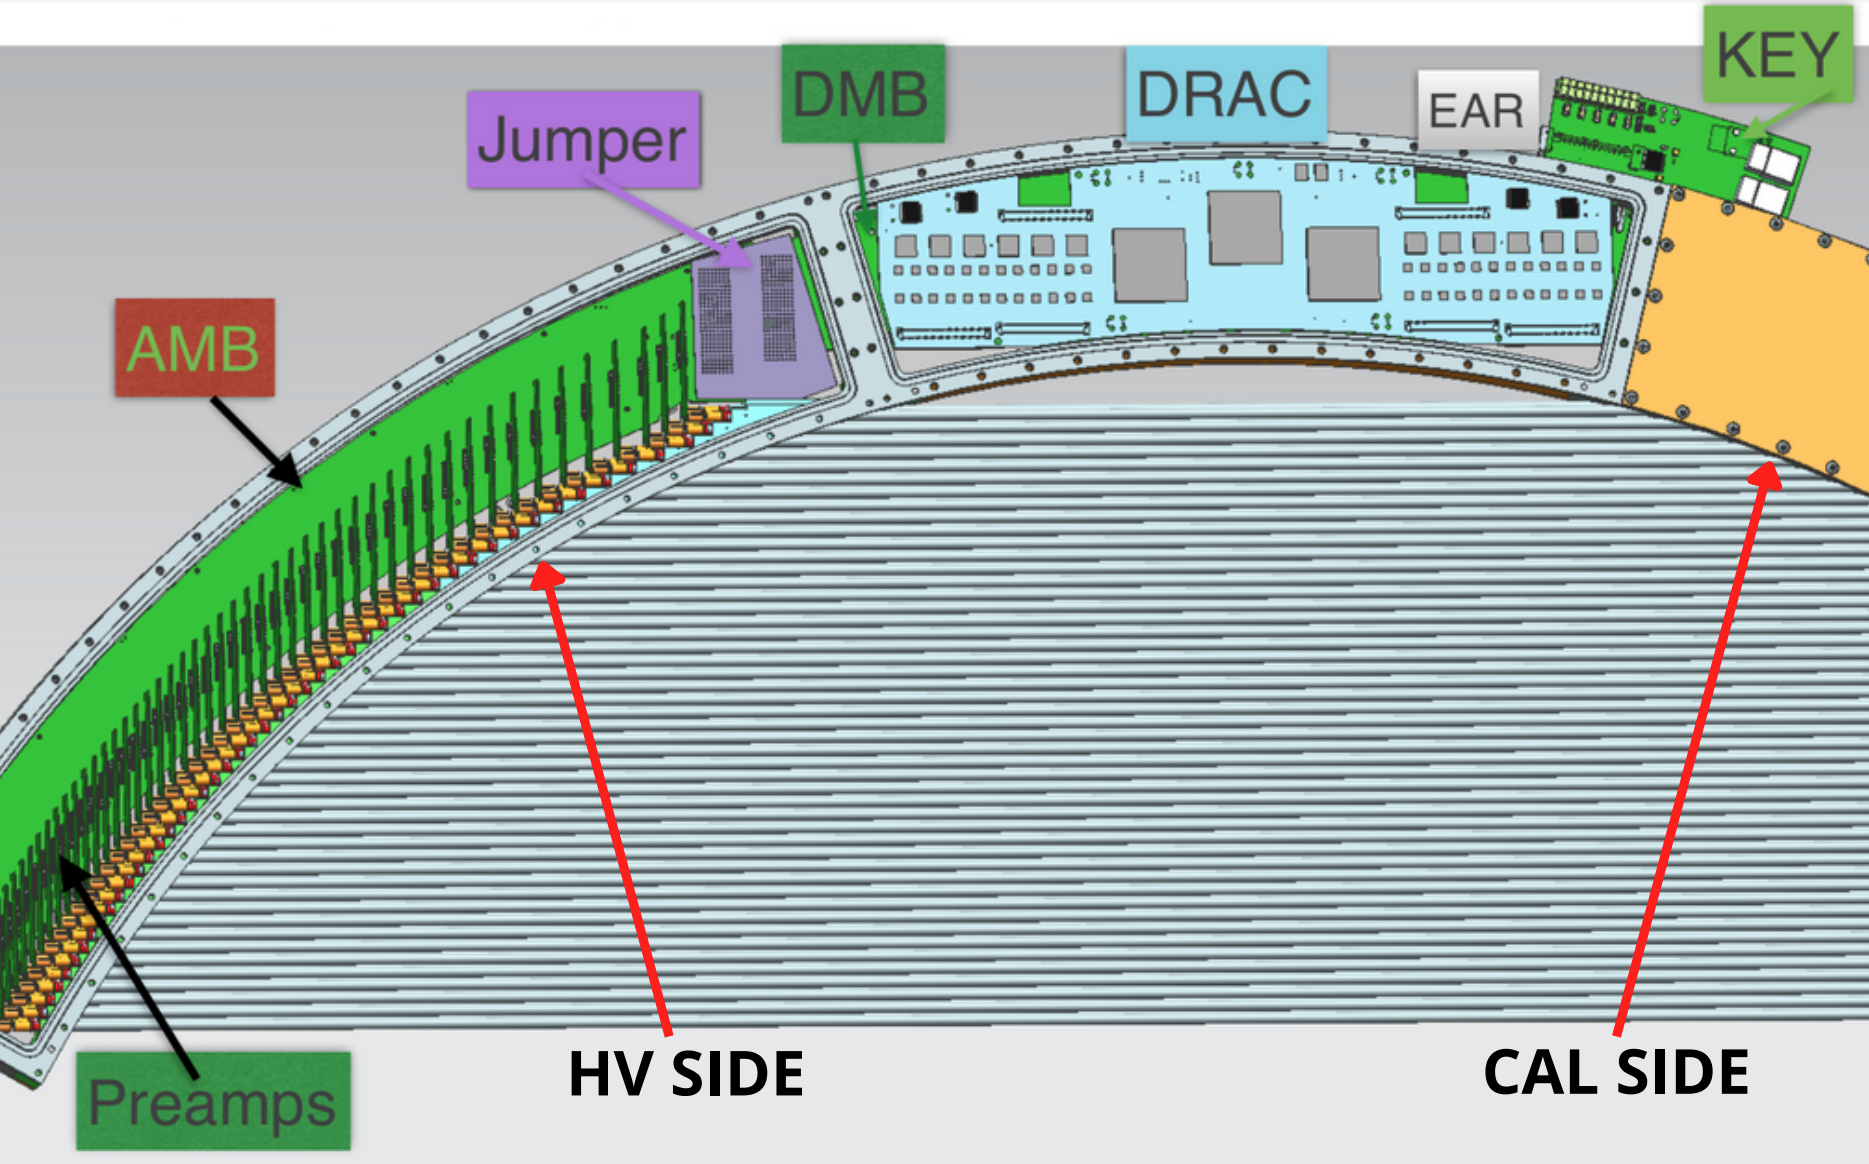
\includegraphics[width =0.8\textwidth]{images/chapter3/Screenshot_20240131_111836.png}
\caption{An overview of the Tracker front-end electronics (FEE) \cite{vadimmu2e}. The preamps and the Analog Motherboard (AMB) on the other side of the straws are not shown in the figure.}
\label{fig:trackerfee}
\end{figure}
On either side, there are an Analog Mother Board (AMB) and a Jumper board, which task consist of directing signals from the preamps towards the Digital Motherboard (DMB) positioned at the center, then to the Digitizer Readout and Assembler Controller (DRAC) (mounted on top of the DMB) to be processed and temporarily stored. Both the AMBs and the DMB handle low voltage distribution and the HV side of the AMB distributes high voltage to the straw anode wires, reason why it is called this way. On the AMBs and the DMB there are sensors, monitoring environmental variables such as temperature, pressure and humidity. The low voltage power supply is fed into the panel through the KEY. The KEY contains an optical fiber link and a JTAG interface for communication. The frontends components were chosen to sustain high level of radiation.
\subsection{Pre-Amplifiers}
The pre-amplifiers (preamps) are responsible for the initial readout of signals from both ends of the straw tube channels. As previously explained, the channels are read out from both ends and two adjacent channels are linked to the same preamp. Each tracker panel contains 48 preamps on the HV side, while an additional 48 preamps are located on the opposite side, the CAL one. Preamps are mounted vertically on the AMBs. Preamps are required to have a matching 300 $\Omega$ input impedance with the straw, in order to avoid signal reflections. The preamps convert the straw tube current signals into voltage signals. Signals are amplified and shaped. The preamps on the CAL and HV sides aren't exactly the same. The CAL preamps have circuitry that can inject calibration pulses into the channel. This capability enables the channel readout electronics to be tested without a high voltage source. The preamps on the HV side distribute the high voltage supply to individual straw tubes. 
%The voltage gains of individual channels, different from the gas gain, are set by control signal from the DRAC. A bias voltage, adjustable for each side of a channel, is applied to the signals. 
\subsection{Digitizer Readout and Assembler Controller}
The brain of a tracker panel is called Digitizer Readout and Assembler Controller (DRAC). The DRAC is responsible for digitizing, packaging and temporary storage. It also controls panel operations. The schematics of the DRAC board is shown in Figure \ref{fig:drac}. In this figure Analog to Digital Converters (ADCs), DDR3 memories and compators are shown. The large chips in the centers are the Field-Programmable Gate Arrays (FPGAs). The one in the center is the Readout Controller (ROC), which manages communications, monitors slow control variables and controls panel operations \ref{ROC}. The left and the right ones, which are referred to as the DIGI FPGAs, are responsible for monitoring data output, buffering data and assembling data packages. Each of them refers to 48 straw channels. 
\begin{figure}[!h]
\centering
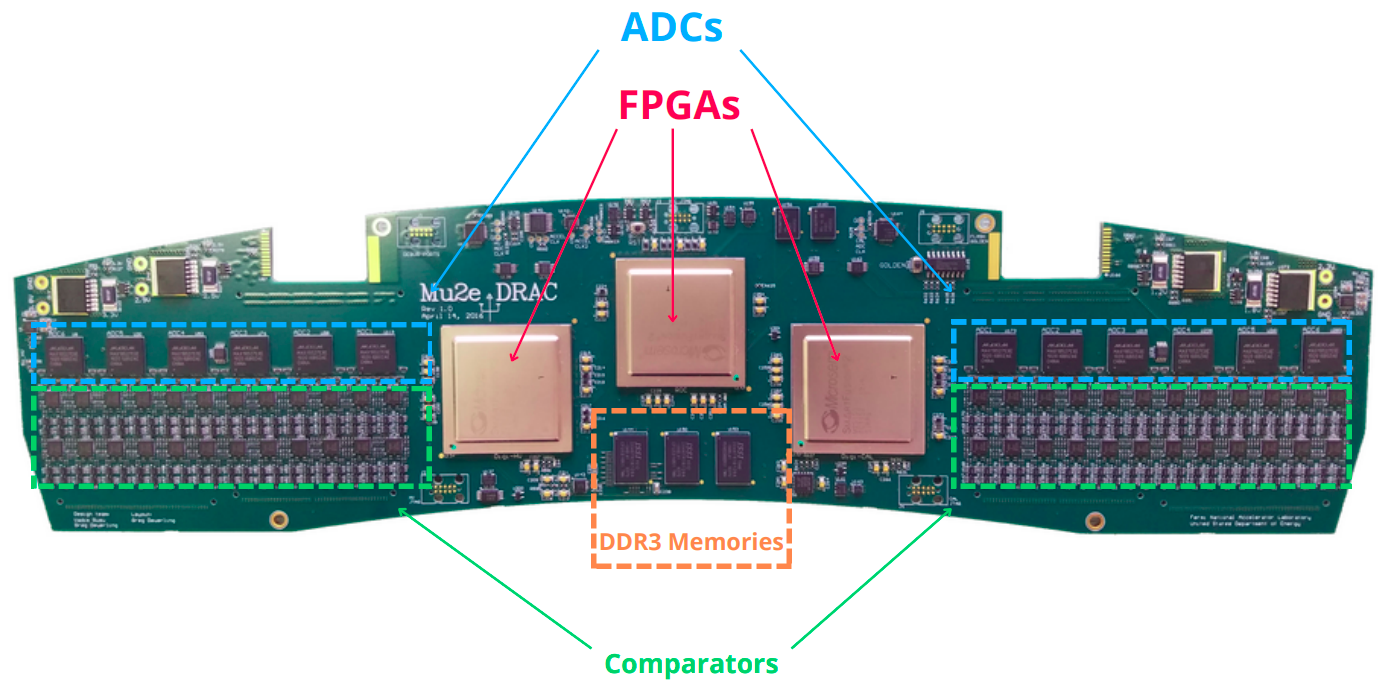
\includegraphics[width =\textwidth]{images/chapter3/Screenshot_20240204_115052.png}
\caption{Digitizer Readout and Assembler Controller (DRAC) board schematics \cite{drac}. The DRAC board is the brain of the tracker panel. In this figure Analog to Digital Converters (ADCs), FPGAs, DDR3 memories and compators are shown.}
\label{fig:drac}
\end{figure}
In figure \ref{fig:flowfee}, signal flow in the Tracker FEEs is reported. At the beginning the signal coming from both ends of the straw is routed to the preamps. After that, the analog signal is sent through the microstrip transmission line to the digitizers. In the DRAC, the two biased signals are fed independently to zero-crossing comparators, which produce square pulses when the signals exceed their respective thresholds. The squared pulses are sent to Time-to-Digital Converters (TDCs, firmware based, 16 bits each) implemented in the DIGI FPGAs, that have the task of digitizing the trigger timings, including the arrival time and the time over threshold, at a rate of about 62.5 MHz. Besides drift time, TDCs measure time difference across the straw to estimate position along the wire and the intrinsic time resolution of TDC is about 25 ps, adding comparator jitter, noise and other external effects the final resolution is $\sim$ 70 ps for time division. Furthermore, an integrator adds voltage signals coming from the two straw ends. In data collection, a hit occurs when both ends of a straw channel are simultaneously activated. The total is digitized by a 12-bit (10-bit ENOB) ADC at 50 MHz and then sent to the DIGI FPGA. The DIGI FPGA creates a data packet for each hit based on TDC and ADC information. This suppresses false triggers caused by random electrical noise. The Digitizer receives signals from both ends of four straws and multiplexes them into one output buffer before sending a packet of data to the ROC. Signals are sent to the ROC at 200 MHz. The data packets are then briefly stored in DDR3 memory for further use by the DAQ system. It is important to save also the voltage signal, since the pulse height information can help us to reject proton background, a significant source of noise or to distinguish muons from electrons. The proton signal will appear as a saturated flag, since the proton $dE/dx$ is $\times$50 the electron one.
\begin{figure}[!h]
\centering
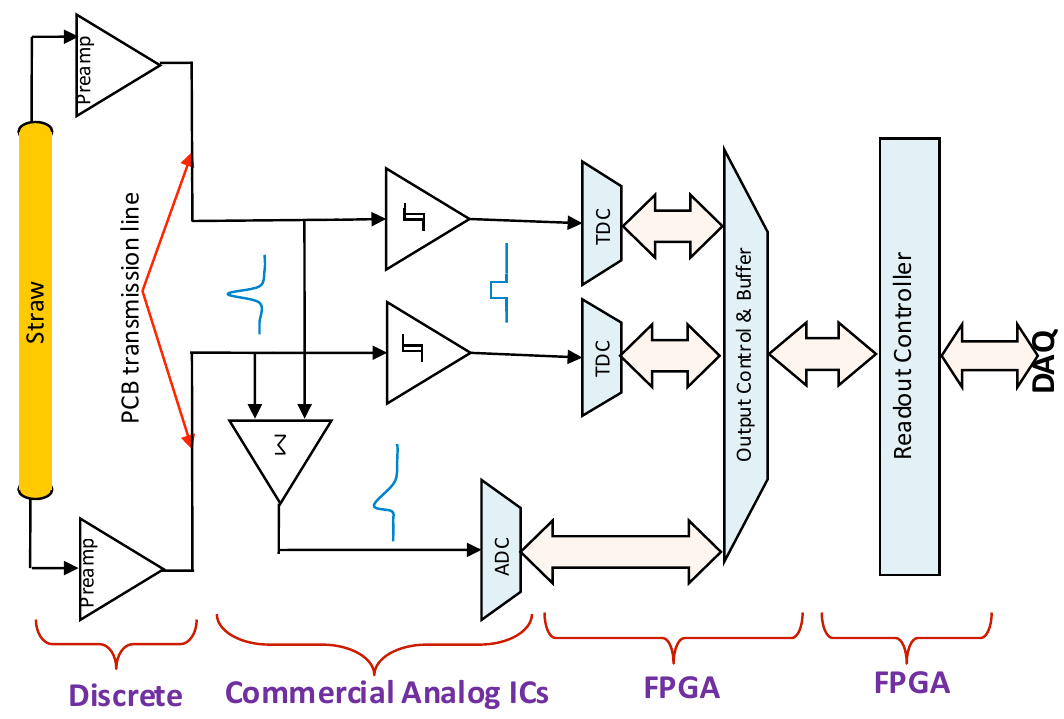
\includegraphics[width =0.8\textwidth]{images/chapter3/Screenshot_20240203_135048.png}
\caption{Signal flow through front end electronics \cite{bartoszek2015mu2e}.}
\label{fig:flowfee}
\end{figure}

\subsection{Read-Out Controller}\label{ROC} 
The main job of the ROCs (one per panel, 216 in total) is to collect data from the digitizer boards, buffer data and send them to DAQ. They are based on an FPGA architecture. They continuously streams out the zero-suppressed data collected between two proton pulses from the detectors, in this case the tracker, to the DTCs (Data Transfer Controller)\cite{GIOIOSA2023167732}. The buffer stage is fundamental, since during the beam inter-spill time (836 ms out of each 1333 ms), we want us to be able to take data from cosmic rays, even if the rate will be very low. For this purpose, the ROCs include external DRAM. The communication is flexible, thanks to the programmable nature of digitizer, ROC and DAQ. 

XXXX immagine 
